\documentclass[11pt]{article}
\usepackage[margin=1in]{geometry}
\usepackage{amsmath,amssymb}
\usepackage{lmodern}
\usepackage[T1]{fontenc}
\usepackage{enumitem}
\usepackage{microtype}
\usepackage{tikz}
\usetikzlibrary{arrows.meta,angles,quotes,calc,decorations.pathreplacing}

\title{2010 F=ma Exam Review}
\author{Nathan P.}
\date{December 22, 2025}

\begin{document}
\maketitle

\section*{Problem 6}
A shortcut: if there was no gravity, $H$ would be double, so $\tan\theta=\dfrac{2H}{R/2}=\dfrac{4H}{R}$, so $\dfrac HR=\dfrac14\tan\theta$. But you can't rely on memorizing facts like that.
You can use the kinematics formulas instead: $H=\dfrac{v^2\sin^2\theta}{2g}$ and $R=\dfrac{v^2\sin2\theta}{g}$, so
\[
\frac HR=\frac{\sin^2\theta/2g}{2\sin\theta\cos\theta/g}=\frac14\tan\theta.
\]

\section*{Problem 13}
For these problems where energy is involved, label your states 1, 2, 3. $E_1=E_2=E_3$:
\[
mgh=\tfrac12mv^2+\tfrac12I\omega^2=\tfrac12I\omega^2+mgy.
\]
It asks for $y$ in terms of $h$, which means we need to solve for $y/h$.
We don't know what $v$ or $\omega$ is, but we can use $v$ to relate $h$ and $y$, because $mgy=mgh-K_{\text{rot}}$, as we can see from energy conservation.
A useful conversion: $K_r=\tfrac12I\omega^2=\tfrac12\cdot\tfrac25mr^2\cdot\dfrac{v^2}{r^2}=\tfrac15mv^2$ for a solid sphere rolling without slipping. In general, for anything rolling without slipping, $K_{\text{rot}}=\tfrac12Cmv^2$, where $C$ is the fraction in front of the rotational inertia.

\section*{Problem 17}
Potential energy comes in pairs.
Count all possible pairs in the arrangement, not just the number of connections one mass can make.
That would be 6 unique pairs, each with $-Gm^2/a$ potential, so just multiply by 6. This number of unique pairs is also equal to the number of edges.

\section*{Problem 18}
Don't forget the negative in $F=-dU/dx$. The negative just means that a positive force is directed in the direction that lessens the potential (for example, radially inward towards a planet). A negative force (in this positive $x$ direction) would increase the potential.
$F=-dU/dx$; in other words, the negative of the slope of the $U$-$x$ graph. Looking at the answer options, $F$-$x$ should be a positive constant when $U$-$x$ has a negative constant slope, and vice versa.

\section*{Problem 19}
The $U$-$x$ and $x$-$t$ graphs are related by $x$. $U$-$x$ just shows the potential at different positions. $x$-$t$ actually shows what positions it progresses through as time goes by.
\begin{itemize}[leftmargin=*, itemsep=0.25em]
\item I works because at $x=15$, $F=-dU/dx=0$, so the object can remain at rest.
\item II doesn't work because at $x=-5$, $F=-dU/dx>0$, so the object cannot remain at rest.
\item III works because from $x=10$ to $x=15$, $F=-dU/dx=0$, so a constant slope ($v$ constant) works, because $F=0$ means $a=0$.
\end{itemize}

\section*{Problem 20}
Total energy is conserved because no non-conservative forces are mentioned.
$E=K+U$, and $K=0$ when $v=dx/dt=0$, so identify the turning points in the $x$-$t$ graph to find $U_{\max}=E_{\text{total}}$.
When $x=5$, $dx/dt=0$ and $U=-5$, so $E_{\text{tot}}=-5$ J.

\section*{Problem 21}
Gravitational self potential energy $\propto M^2/R$ (in fact, for a uniform sphere, $U=\tfrac35GM^2/R$).
$M\propto R^3$, so $U\propto R^6/R\propto R^5$, so $2R\to 32U$.

\section*{Problem 23}
\[
\Delta m=\rho V=\rho AL=\rho Av\Delta t,\qquad
\Delta p=\Delta m\,\Delta v=\Delta m(-2v)=-2\rho Av^2\Delta t,\qquad
F=\frac{\Delta p}{\Delta t}=-2\rho Av^2.
\]
$\sum F=0$, so $F_1=F_2$: $-2\rho Av^2=-2\rho\dfrac A2v'^2$, so $v'=v\sqrt2$.

\section*{Problem 24}
$I_0=\tfrac12MR^2$. The $I$ of the $R/2$ cutout (about the axis):
\[
I=\tfrac12\cdot\tfrac14M\left(\tfrac R2\right)^2+\tfrac14M\left(\tfrac R2\right)^2=\tfrac1{32}MR^2+\tfrac1{16}MR^2=\tfrac3{32}MR^2.
\]
The cutout is $\tfrac14M$ because $M\propto R^2$.
\[
I_0-I=\left(\tfrac{16}{32}-\tfrac3{32}\right)MR^2=\tfrac{13}{32}MR^2.
\]
Strategy: $I$ of the original disk minus $I$ of the cutout about an axis through its edge.

\begin{center}
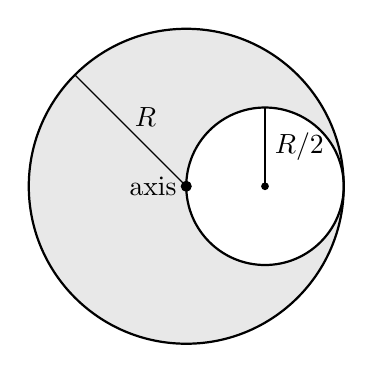
\begin{tikzpicture}[scale=1.0, line cap=round, line join=round, >={Stealth[length=2mm]}]
  \fill[gray!18, even odd rule] (0,0) circle (2) (1,0) circle (1);
  \draw[thick] (0,0) circle (2);
  \draw[thick] (1,0) circle (1);
  \fill (0,0) circle (2pt) node[left] {axis};
  \draw (0,0) -- (-1.414,1.414) node[midway, above right=-2pt] {$R$};
  \draw (1,0) -- (1,1) node[midway, right] {$R/2$};
  \fill (1,0) circle (1.4pt);
\end{tikzpicture}
\end{center}

\section*{Problem 25}
Many F=ma problems ask for new in terms of old. It's evident when the answer options are all in terms of the old variable: speed, time, height, you name it.
\begin{enumerate}[leftmargin=*, itemsep=0.25em]
\item Identify what the question wants: $v/v_0$. So we need expressions for both new and old.
\item Express the new first, so we know what to express the old in terms of.
\item Can we express the old in terms of the same variables? If yes, carry out the physics.
\item Last step: divide new by old and obtain the answer!
\end{enumerate}
\[
v^2=\frac{GM}{2R},\qquad
v_0^2=GM\left(\frac2r-\frac1a\right)=GM\left(\frac2{2R}-\frac2{3R}\right)=\frac{GM}{3R},
\]
\[
\frac{v^2}{v_0^2}=\frac{1/2}{1/3}=\frac32,\qquad v=\sqrt{\tfrac32}\,v_0.
\]

\end{document}
